
\documentclass[11pt,a4paper,slovene]{myarticle}

%Uporabljeni paketi
\usepackage[slovene]{babel}
\usepackage[utf8]{inputenc}
\usepackage{lmodern}
\usepackage[T1]{fontenc}
\usepackage{fancyhdr}
\usepackage{caption}
\captionsetup{font={default,footnotesize}, labelfont=bf, format=hang,indention=.0cm}
\usepackage{graphicx,epsfig}
\usepackage{amsmath}
\usepackage{multirow}
\usepackage{color}
\usepackage{url}
\usepackage{makeidx}
\usepackage[official]{eurosym}

\usepackage{hyperref}
\hypersetup{
   bookmarksnumbered=true,
   urlbordercolor={0 1 0},
   linkbordercolor={1 1 1},
   unicode=true,
   pdftitle={ Modeliranje Računalniških Omrežij },
   pdfauthor={Aljaž Markežič, Žan Valter Dragan},
   pdfdisplaydoctitle=true,
   pdftoolbar=true,
   pdfmenubar=true,
   pdfstartview=X Y Z
}

\urlstyle{same}

\setlength{\parskip}{12pt}
\setlength\parindent{0pt}
\setlength\unitlength{1mm}

\begin{document}
\label{naslov}
\pdfbookmark[1]{Naslov}{naslov}
\thispagestyle{empty}

\begin{center}
\begin{Large}
Modeliranje računalniških omrežij\\
Študijsko leto 2016/2017\\
\end{Large}

\vspace*{4cm}
\begin{LARGE}
\textbf{Implementacija IEEE 802.11 v orodju OMNeT++\\}
\end{LARGE}
\vspace*{0.5cm}

\begin{Large}
Modeliranje brezžičnih omrežij\\

\vspace*{4cm}

Aljaž Markežič, Žan Valter Dragan\\
Vpisna št. 63140157, 63140045\\

\vspace*{5cm}
Ljubljana, \today
\end{Large}
\end{center}

\pagebreak
\setcounter{page}{1}
\pagenumbering{arabic}


\label{Kazalo}
\pdfbookmark[1]{Kazalo}{Kazalo}
\tableofcontents
\thispagestyle{empty}
\pagebreak

\section{Uvod in motivacija}
V zadnjih letih se je zelo razširila nova doba povezljivosti, tako imenovani Internet of Things (IoT) oziroma Internet Stvari. Trg v omrežje povezanih naprav se neprestano povečuje z nezanemarljivo hitrostjo. Ker so kabli preokorni in Bluetooth ni vedno optimalen, se velikokrat išče rešitev v brezžičnih povezavah tipa IEEE 802.11. V tej seminarski nalogi se bova osredotočila na te povezave in jih nekaj tudi bolj nadrobno predstavila. Simulirala bova različna omrežja in preverila, kako se posemezen tip odnese. S tem bova pridobila podatke, kateri se nato lahko uporabijo pri izdelavi povezanih naprav.

\section{Opis specifikacij IEEE 802.11}
Zametki standarda IEEE 802.11 segajo že v leto 1985, vendar se je specifikacijo standardiziralo šele leta 1997. V 802.11 sta zajeti fizična plast ter del podatkovne plasti (Media Access Control - MAC). Standard se preko revizij spreminja še sedaj. Prva bolje zastopana različica je bila 802.11b, nekaj drugih pa je še a, g, n, ac, ... Ti standari delujejo na frekvencah 900MHz, 2.4GHz, 3.6GHz, 5GHz ter 60GHz. Naprave z 2.4GHz implementacijo občutijo občasne motnje drugih naprav, kot so mikrovalovne pečice, Bluetooth naprave in druge. Motnje rešujemo z raznimi modulacijami (Direct-Sequence Spread Spectrum, Orthogonal Frequency-Division Multiplexing). Povezave običajno dosegajo hitrosti v Mbit/s (od 1 do 866), kar pa so želeli spremeniti s standardom 802.11ad, kjer je možno doseči hitrosti do 7Gbit/s z uporabo višjih frekvenc.

\section{Uporabljene knjižnice}

\subsection{Razpoložljivi gradniki v OMNeT++}
\begin{itemize}
	\item \textbf{IPv4NetworkConfigurator:} modul, ki napravam v omrežju dodeli ipv4 naslove, ter skrbi za statično usmerjanje v omrežju. Modulu lahko nastavljamo naslednje atribute: address, netmask, multicast group, mtu,…
	\item \textbf{WirelessHost:} modul, ki simulira delovanje IP gostitelja (host-a), torej je sposoben posredovat, sprejemat in odgovarjat na sporočila, ki se pretakajo po omrežju. Nekaj od atributov ki jih lahko nastavljamo temu modulu so: bandwith,  transmiter.power, carierFrequency, reciever.sensiticity, antenaGain,…
	\item \textbf{Radio Medium:} modul, ki opisuje model deljenega fizičnega medija preko katerega potekajo vse komunikacije v omrežju. Modulu lahko določamo razne atribute kot so: material, backgroundNoise, pathloss, obstacleLoss,…, s pomočjo katerih lahko simuliramo dejanski medij preko katerih bi potekala brezžična povezava
	\item \textbf{PhysicalEnvironment:} modul, ki simulira fizične ovire, ki se lahko znajdejo v testnem okolju. S pomočjo tega modula lahko simuliramo kako se bo odzivalo omrežje, saj fizične ovire vplivajo na porabo energije, ter premikanje brezžičnih gostiteljev (wirelessHosts). Modulu lahko nastavljamo naslednje atribute: position, orientation, shape, material, color, opacity
	\item \textbf{AccessPoint:} modul, ki simulira generično vstopno točko (access point), preko katere si lahko naprave izmenjujejo sporočila, ter podpira več brezžičnih frekvenc in ethernet vhodov.
\end{itemize}

\subsection{Zgledi omrežij 802.11 v OMNeT++}
Za delo v okolju OMNeT++ imamo na voljo kar nekaj primerov, med katerimi je tudi ogrodje INET. Ti primeri služija koz prikaz možnih postavitev, kot tudi morebitnih težav, ki se lahko pojavijo znotraj tovrstnih omrežij. V nadaljevanju so predstavljeni trije primeri brezžičnih omrežij.
\subsubsection{Primer1 - LAN 802.11}
Omrežje je definirano v datoteki Lan80211.ned v kateri je predstavljeno omrežje za testiranje 802.11 modela v infrastrukturnem načinu. Omrežje je sestavljeno iz vstopne točke (Access Point – AP) v infrastrukturnem načinu, ter poljubnim številom gostiteljev(host) tipa 	WirelessHost. Konfiguracija omrežja je opisana v datoteki omnetpp.ini v katerem lahko definiramo razne atribute omržeja, kot so: constraintArea(območje kritja AP), MAC naslov AP, gibanje gostiteljev, ... Simulacija (1*AP, 2*HOST) poteka tako, da prvo host[1] pošlje arpReq AP kjer zahteva MAC address za določen IP, AP na sprejeto sporočilo odgovori z ACK, ter nato broadcasta ta arpReq vsem ostalim napravam v območju kritja. Ko ciljna naprava dobi ARPReq, pošlje AP nazaj ARPReply, ta pa mu nazaj odgovori z ACK. Potem AP broadcasta 	ARPReply vsem napravam v dosegu. Ko ciljna naprava dobi paket odgovori nazaj z ACK, kar pomeni da sedaj host[1], ve MAC naslov naprave za IP naslov, ki ga je zahteval v ARPReq. Tako se lahko začne komunikaciaj med host[1] pa host[0], kar je v simulaciji izvedeno preko ICMP ping paketov.
\begin{figure}[h!]
	\centering
		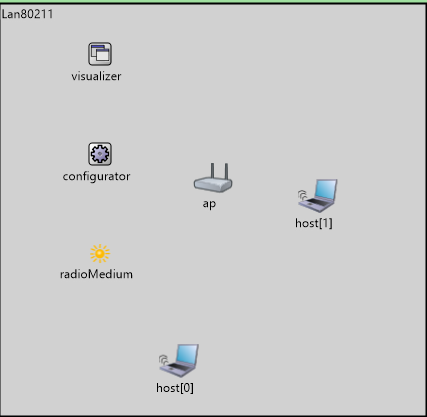
\includegraphics[width=0.9\textwidth, keepaspectratio=true]{./images/lan80211.png}
	\caption{LAN 802.11}
	\label{fig:lan80211}
\end{figure}

\subsubsection{Primer2 - QOS}
Omrežje je definirano v datoteki Throughput.ned v kateri je predstavljeno omrežje, ki simulira celotno vzpostavitev povezazve med gostiteljem(hostom), ter strežnikom(server), ki sta oba tipa WirelessHost preko vstopne točke (Access Pointa – AP), ki je tipa AccessPoint. Konfiguracija omrežje je opisana v datoteki omnetpp.ini kjer lahko spreminjamo iste paramtere kot v prejšnjem primeru, torej: constraintArea(območje kritja AP), MAC naslov AP, ... Simulacija se začne tako da AP pošilja Beacon pakete s katerimi se oglašuje, oziroma poziva naprave da se povežejo nanj. Če se naprave želijo povezati na AP to storijo Probe Request paketom, na kar AP 	odgovori z Probe response paketom. Nato so začne faza avtentikacije, asociacije in ARP discovery faza, kjer si AP in gostiteljske naprave izmenjenajo razne podatke za vzpostavitev povezave. Ko je gostiteljska naprava dokončno vzpostavila povezavo z AP, se začne komunikacija med strežnikom in odjemalcem, kjer odjemalec zahteva različne pakete kot so, Video, WWW, FTP, ...
\begin{figure}[h!]
	\centering
		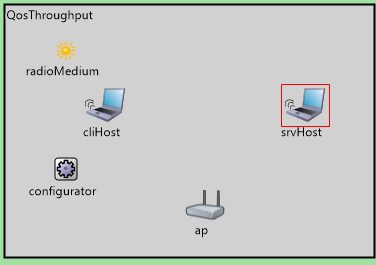
\includegraphics[width=0.9\textwidth, keepaspectratio=true]{./images/qos.png}
	\caption{QOS}
	\label{fig:QOS}
\end{figure}

\subsubsection{Primer3 - Synchronized}
\begin{figure}[h!]
	\centering
		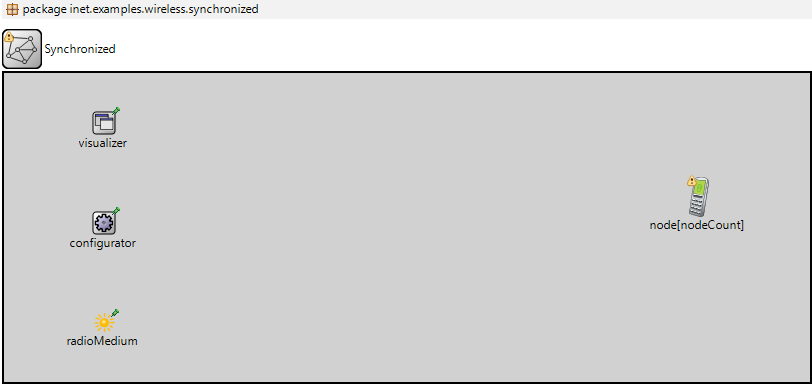
\includegraphics[width=0.9\textwidth, keepaspectratio=true]{./images/syn-components.png}
	\caption{Synchronized - Gradniki}
	\label{fig:synchronizedgradniki}
\end{figure}
Ta primer prikaže morebitne napake, katere se pojavijo ob sinhronem oddajanju signalov večih naprav znotraj brezžičnega omrežja. Na voljo imamo sledeča gradnika: radioMedium in node. Naprave oddajajo UDP pakete v ad hoc omrežje sinhrono - vedno pošiljajo ob istem času. Le-to povzroči izgubo paketov zaradi medsebojnih motenj valovanj. To razrešimo z vpeljavo naključnih zakasnitev na aplikacijski ravni, kar pomeni, da omrežje postane asinhrono.

V simulacijskih nastavitvah je možno nastaviti število naprav (privzeta vrednost je 30), ter območje znotraj katerega se nahajajo. Na voljo sta tudi dve konfiguraciji - sinhrona in asinhrona, kjer nastavimo čas pošiljanja paketov. Pri asinhroni konfiguraciji je na voljo tudi nastavitev tipa MAC naslova, katera pa je privzeto zakomentirana.
\begin{figure}[h!]
	\centering
		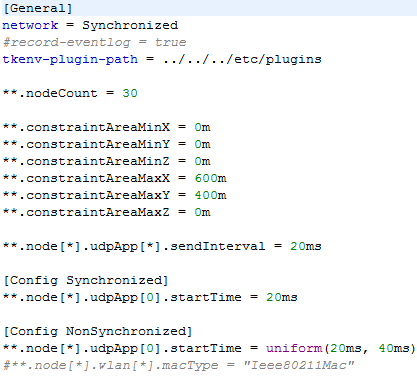
\includegraphics[width=0.9\textwidth, keepaspectratio=true]{./images/syn-settings.png}
	\caption{Synchronized - Nastavitve Simulacije}
	\label{fig:synchronizednastavitvesimulacije}
\end{figure}
\begin{figure}[h!]
	\centering
		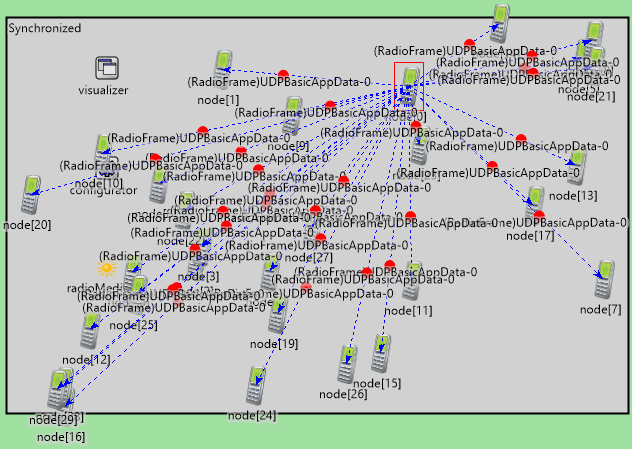
\includegraphics[width=0.9\textwidth, keepaspectratio=true]{./images/syn-simulation.png}
	\caption{Synchronized - Simulacija}
	\label{fig:synchronizedsimulacija}
\end{figure}

\pagebreak

\section{Rešitev}

\subsection{Načrtovanje omrežij}
V prejšnjih poglavjih smo predstavili gradnike, s pomočjo katerih bomo realizirali 4 različna omrežja, ter predstavili že pripravljene primere iz knjižnice INET, kateri so nam služili kot izhodišče za postavitev lastnih omrežij.
\begin{itemize}
	\item Omrežje 1: preprosto brezžično omrežje z vstopno točko in dvema gostiteljema.
	\item Omrežje 2: vstopna točka z dvema gostiteljema in betonsko oviro.
	\item Omrežje 3: predstavlja domačo omrežje z dvema sobama.
	\item Omrežje 4: predstavlja bolj zapleteno omrežje z več vstopnimi točkami. Gostitelji so razporejeni v prostorih ob hodniku.
\end{itemize}

\pagebreak

\subsubsection{Omrežje 1}
Ideja tega omrežja je opazovanje obnašanja brezžičnega omrežja v idealnem okolju (dober signal, brez ovir in nasičenosti). Izhodišče predstavlja primer lan80211 s spremenjenimi parametri. Sestavlja ga ena vstopna točka, ter dva gostitelja.
\begin{figure}[h!]
	\centering
		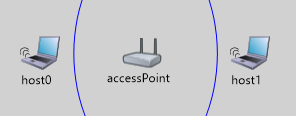
\includegraphics[width=0.7\textwidth, keepaspectratio=true]{./images/om1-layout.png}
	\caption{Omrežje 1 - postavitev}
	\label{fig:om1layout}
\end{figure}

\subsubsection{Omrežje 2}
To omrežje izhaja iz prvega omrežja, kateremu sva dodala vertikalni betonski zid. S tem sva dobila podatke, kako se omrežje obnaša v neidealnem omrežju, kar sva uporabila kot referenco za naslednja omrežja. Drugo omrežje sestavljajo vstopna točka, dva gostitelja in vertikalna betonska ovira.
\begin{figure}[h!]
	\centering
		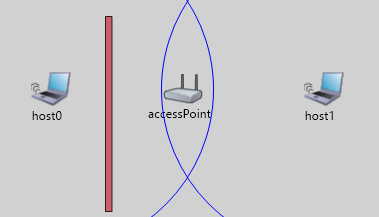
\includegraphics[width=0.7\textwidth, keepaspectratio=true]{./images/om2-layout.png}
	\caption{Omrežje 2 - postavitev}
	\label{fig:om2layout}
\end{figure}

\subsubsection{Omrežje 3}
Tretje omrežje predstavlja primer postavitve domačega omrežja, kjer so sobe ločene s steklenimi zidovi, zunanji pa so betonski. V srednji sobi je postavljena vstopna točka, v sobah na levi in desni strani pa sta v vsaki po en gostitelj. Ravno tako je en gostitelj postavljen izven stanovanja. S tem omrežjem sva pridobila podatke, kako se brezžično omrežje obnaša v pogojih z različnimi ovirami.
\begin{figure}[h!]
	\centering
		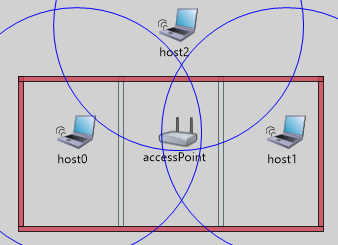
\includegraphics[width=0.7\textwidth, keepaspectratio=true]{./images/om3-layout.png}
	\caption{Omrežje 3 - postavitev}
	\label{fig:om3layout}
\end{figure}

\pagebreak

\subsubsection{Omrežje 4}
Pri postavitvi četrtega omrežja sva imela v mislih učilnice razporejene ob hodniku. V primerjavi s prejšnjim omrežjem se tu nahaja več gostiteljev in več fizičnih ovir. Ravno tako se omrežje nahaja na večji površini, kar pomeni, da ena vstopna točka ne bi bila dovolj. Stene med učilnicami so betonske, medtem ko mejne s hodnikom steklene.
\begin{figure}[h!]
	\centering
		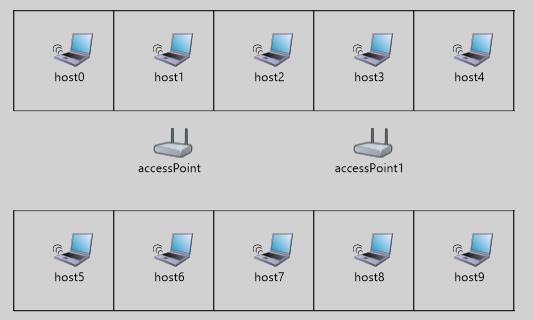
\includegraphics[width=0.9\textwidth, keepaspectratio=true]{./images/om4-layout.png}
	\caption{Omrežje 4 - postavitev}
	\label{fig:om4layout}
\end{figure}

\section{Simulacije in rezultati}
Za izvajanje simulacij sva izbrala 5 parametrov, ki vplivajo na delovanje omrežja in 3 metrike preko katerih lahko določimo učinkovitost posameznega omrežja.

\textbf{Parametri:}
\begin{itemize}
	\item *.host*.wlan[0].radio.transmitter.power:
		\subitem enota miliVati (mW)
		\subitem parameter določa moč s katero gostitelj oddaja signal
	\item *.host1.pingApp[0].sendInterval:
		\subitem enota milisekunde (ms)
		\subitem parameter določa hitrost pošiljanja paketov
	\item *.radioMedium.backgroundNoise.power:
		\subitem enota decibel-miliVat (dBm)
		\subitem parameter določa jakost okoljskega šuma
	\item *.accessPoint.**.sensitivity
		\subitem enota decibel-miliVat (dBm)
		\subitem parameter določa prag, nad katerim mora biti moč signala, da vstopna točka lahko prejme podatke
\end{itemize}

\textbf{Metrike:}
\begin{itemize}
	\item Round Trip Time (RTT): čas, ki ga poslan paket potrebuje, da pride od izvora do ponora, ter nazaj
	\item pingLossRate: razmerje med številom poslanih ter izgubljenih paketov
	\item Signal to Noise plus Interference Ratio (SNIR): razmerje med močjo signala ter vsoto moči šuma in interference ostalih signalov
\end{itemize}

\textbf{Ovire:}
\begin{itemize}
	\item betonske:
		\subitem omrežji 2 in 3: širina stene 1m
		\subitem omrežje 4: širina stene 0,3m
	\item steklene:
		\subitem omrežje 3: širina stene 1m
		\subitem omrežje 4: širina stene 0,2m
\end{itemize}

Za protokol, preko katerega bodo komunicirali gostitelji, sva si izbrala ICMP paket ping. Razlog za izbiro je predvsem v preprostosti, poleg tega ping preverja, ali smo dobili odgovor od naslovnika.

Samo načtrovanje simulacije je potekalo tako, da sva najprej poiskala srednje vrednosti, v katerih omrežja niso imela prevelikih izgub, a vseeno niso delovala idealno. Nato pa sva jih spreminjala in opazovala spremembe pri rezultatih.

\subsection{Omrežje 1}
\begin{table}[h]
	\centering
		\begin{tabular}{| l | l | l | l | l | l |}
			\hline
			Metrika / Moč[mW] & 80 & 85 & 90 & 95 & 100 \\
			\hline
			RTT[ms] & 33,00 & 3,09 & 0,50 & 0,29 & 0.25 \\
			\hline
			PingLossRate[\%] & 77,00 & 13,34 & 26,25 & 27,73 & 27,00 \\
			\hline
			SNIR[dB] & 94,00 & 99,58 & 105,00 & 111,77 & 117,00 \\
			\hline
		\end{tabular}
	\caption{Omrežje 1 - rezultati}
	\label{tab:om1rezultati}
\end{table}
Opazimo, da smo najboljše vrednosti metrik dobili pri moči signala 85mW.
Ob nižji moči se kvaliteta omrežja poslabša, kar namiguje na pomembnost moči signala pri brezžičnih omrežjih. Z nizko močjo se poveča čas potovanja paketa, ter večje izgube le-teh.
Z večjo močjo pa se povečajo tudi interference, kar nam sicer zmanjša čas potovanja paketa, a hkrati poveča izgubo. Zato bi se tukaj morali odločiti, če nam je pomembnejša hitrost, ali gotovost dostave.

\subsection{Omrežje 2}
\begin{table}[h!]
	\centering
		\begin{tabular}{| l | l | l | l | l | l |}
			\hline
			Metrika / Moč[mW] & 50 & 60 & 70 & 80 & 90 \\
			\hline
			RTT[ms] & 41,00 & 13,00 & 0,23 & 0,22 & 0.22 \\
			\hline
			PingLossRate[\%] & 98,97 & 38,99 & 30,00 & 30,00 & 30,00 \\
			\hline
			SNIR[dB] & 115,00 & 117,00 & 121,00 & 121,00 & 156,24 \\
			\hline
		\end{tabular}
	\caption{Omrežje 2 - rezultati}
	\label{tab:om2rezultati}
\end{table}
Zaradi postavljene stene je bilo potebno zmanjšati šum (iz -90dBm na -100dBm), sicer signal sploh ni prišel čez.
Pri tem omrežju je bila najboljša moč 90mW, katera je hkrati tudi največja.
Veliko vlogo pri rezultatih ima postavljena ovira, katera povzroča precejšnjo izgubo paketov. Kljub temu se čas potovanja pri višji moči ni poslabšal.

\subsection{Omrežje 3}
S tretjim omrežjem sva vpeljala različne vrste materialov, kar sva tukaj tudi primerjala.

\subsubsection{Steklena stena}
Najprej sva poiskala potrebno konfiguracijo za potek komunikacije preko steklene stene (smer host1 - host0).

\begin{table}[h!]
	\centering
		\begin{tabular}{| l | l |l | l |}
			\hline
			 & \multicolumn{3}{| c |}{Metrike} \\
			\hline
			Smer & RTT[ms] & PingLossRate[\%] & SNIR[dB] \\
			\hline
			host1 - host2 & NaN & 100 & 164 \\
			\hline
			host1 - host0 & 0,50 & 4,50 & 164 \\
			\hline
		\end{tabular}
	\caption{Omrežje 3 (steklo) - rezultati}
	\label{tab:om3steklorezultati}
\end{table}

Moč pri simulaciji s stekleno steno je bila za vse gostitelje enaka, in sicer 16mW, medtem ko je vstopna točka imela 20mW.
Že sedaj rezultati nakazujejo na očitno razliko v izbiri material pri enaki debelini.

\subsubsection{Betonska stena}
Potek komunikacije betonske stene je v smeri host1 - host2.

\begin{table}[h!]
	\centering
		\begin{tabular}{| l | l | l | l |}
			\hline
			 & \multicolumn{3}{| c |}{Metrike} \\
			\hline
			Smer & RTT[ms] & PingLossRate[\%] & SNIR[dB] \\
			\hline
			host1 - host2 & 0,77 & 8,50 & 807 \\
			\hline
			host1 - host0 & 0,64 & 9,00 & 807 \\
			\hline
		\end{tabular}
	\caption{Omrežje 3 (beton) - rezultati}
	\label{tab:om3betonrezultati}
\end{table}

Moč gostiteljev pri tem primeru je bila za host0 in host1 enaka 16mW, ter host2 enaka 100mW, ravno toliko je bila tudi moč vstopne točke.

Iz teh primerov je lepo vidna razlika v uporabi materiala, ko imamo pri manjši moči polno izgubo preko betona, a minimalno preko stekla. Ravno tako je za preboj betona potrebna kar 5-kratna moč, ob čemer opazimo tudi povečano interferenco na povezavi med host0 in host1 v večjem RTT in tudi večji izgubi paketov.

\subsection{Omrežje 4}
To omrežje sva poizkušala čim bolj približati realni situaciji, saj sva želela preveriti metrike v okviru vsakdanjih okoliščin. V ta namen sva spremenila debelino ovir, ter povečala število gostiteljev in vstopnih točk.

Za zagone simulacij sva uporabila sledeče trajne nastavitve:
\begin{itemize}
		\item moč šuma: -100dBm
		\item moč gostiteljev: 100mW
		\item interval pošiljanja: 1s
		\item velikost vrste vstopne točke: 100
\end{itemize}

Poleg trajnih sva spreminjala še nastavitvi moči vstopne točke (VT) in njene občutljivost.
\begin{table}[h!]
	\centering
		\begin{tabular}{| l | l | l |}
			\hline
			Številka zagona & Moč VT[mW] & Občutljivost VT[dBm] \\
			\hline
			1 & 80 & -79 \\
			\hline
			2 & 80 & -89 \\
			\hline
			3 & 90 & -79 \\
			\hline
			4 & 90 & -89 \\
			\hline
		\end{tabular}
	\caption{Omrežje 4 - variabilni parametri}
	\label{tab:om3variabilniparametri}
\end{table}

Po zagnanih simulacijah sva prišla do naslednjih rezultatov:
\begin{itemize}
	\item SNIR: pri vseh zagonih je bil 50dB
	\item Ping Loss Ratio:
		\subitem iz grafa je takoj možno odčitati, da se zagon številka 3 najboljše odreže
		\subitem na tej točki predvidevava, da se bo podobna kvaliteta konfiguracije izkazala tudi pri RTT
		\begin{figure}[h!]
			\centering
				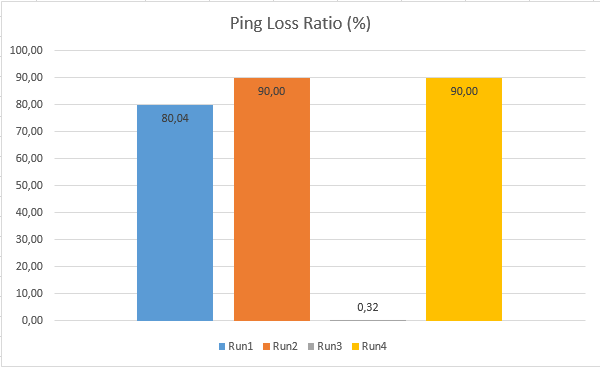
\includegraphics[width=0.9\textwidth, keepaspectratio=true]{./images/om4-ping-mean.png}
			\caption{Omrežje 4 - Ping Loss Ratio}
			\label{fig:om4pinglossratio}
		\end{figure}
	\item RTT:
		\subitem pri tej metriki je treba biti pazljiv, saj ničelni RTT ne pomeni najboljše omrežje, nasprotno, gre za najslabše. Če je ta metrika 0, to pomeni, da odgovor nikoli ni prišel in časa potovanja paketa pravzaprav niti nismo mogli izmeriti. Četudi v splošnem velja, da je manjši RTT željen, je potreben dodaten premislek.
		\begin{figure}[h!]
			\centering
				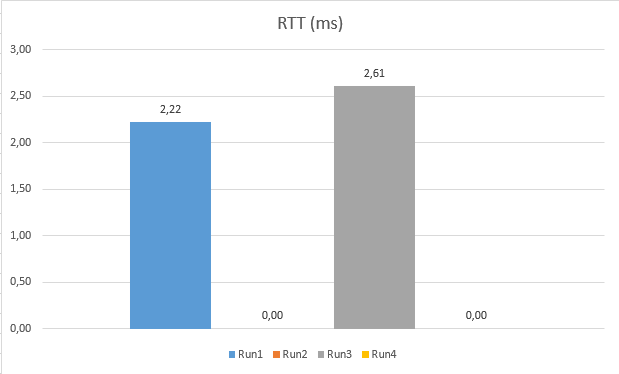
\includegraphics[width=0.9\textwidth, keepaspectratio=true]{./images/om4-rtt-mean.png}
			\caption{Omrežje 4 - RTT}
			\label{fig:om4rtt}
		\end{figure}
\end{itemize}

Iz podanih rezultatov lahko sklepamo, da je konfiguracija drugega zagona najboljša izmed testiranih. Čeprav nima najboljšega RTT-ja, to razliko slabih pol sekunde brez težav vzamemo v zakup pri neprekosljivi zanesljivosti dostave.
Razlog, zakaj sta druga ter četrta zagona imela tako velike težave pri dostavi paketov, sva našla v vrednostih občutljivosti vstopnih točk. Kadar je bila ta vrednost nekoliko bolj negativna (-89dBm), so bile izgube večje. Tako je prvi zagon imel vendarle nekaj uspelih paketov, kljub nižji moči vstopnih točk. Za dobro performanco omrežja pa je poskrbela kombinacija večje moči ter manjše občutljivosti vstopnih točk, kot prikazano z drugim zagonom.

\section{Zaključek}
V tej seminarski nalogi sva dosegla zastavljene cilje, saj sva pridobila podatke, kako se omrežje IEEE 802.11 obnaša v raznih okoliščinah. Predvsem zanimive so se nama zdele relacije med debelino ovir, njihovim materialom, ter močjo signala, kot tudi vpliv šuma in občutljivosti na kakovost omrežja. Ravno tako se je za pomemben faktor izkazalo število uporabnikov v omrežju, saj dokaj hitro pride do kolizij in interference. Vse to bo v prihajajočem razvoju povezanih stvari potrebno še dodatno premisliti in poizkušati najti odgovore na trenutne problematike protokola.

V pomoč pri razumevanju tematike nama je bila tudi uradna dokumentacija orodja OMNeT++\cite{omnetpp}, katero sva uporabila kot referenco za večji del projekta. Ob tem sva dobila tudi nekoliko boljši občutek za potencialni razvoj na področju brezžične tehnologije, katera vse prej kot stagnira\cite{wiki-802.11}.

\pagebreak
\bibliographystyle{plain}
\bibliography{references}

\end{document}







